%%%%%%%%%%%%%%%%%%%%%%% file template.tex %%%%%%%%%%%%%%%%%%%%%%%%%
%
% This is a general template file for the LaTeX package SVJour3
% for Springer journals.          Springer Heidelberg 2010/09/16
%
% Copy it to a new file with a new name and use it as the basis
% for your article. Delete % signs as needed.
%
% This template includes a few options for different layouts and
% content for various journals. Please consult a previous issue of
% your journal as needed.
%
%%%%%%%%%%%%%%%%%%%%%%%%%%%%%%%%%%%%%%%%%%%%%%%%%%%%%%%%%%%%%%%%%%%
%
% First comes an example EPS file -- just ignore it and
% proceed on the \documentclass line
% your LaTeX will extract the file if required
\begin{filecontents*}{GTS_on_net-traffic.eps}
%!PS-Adobe-3.0 EPSF-3.0
%%BoundingBox: 19 19 221 221
%%CreationDate: Mon Sep 29 1997
%%Creator: programmed by hand (JK)
%%EndComments
gsave
newpath
  20 20 moveto
  20 220 lineto
  220 220 lineto
  220 20 lineto
closepath
2 setlinewidth
gsave
  .4 setgray fill
grestore
stroke
grestore
\end{filecontents*}
%
\RequirePackage{fix-cm}
%
\documentclass{svjour3}                     % onecolumn (standard format)
%\documentclass[smallcondensed]{svjour3}     % onecolumn (ditto)
%\documentclass[smallextended]{svjour3}       % onecolumn (second format)
%\documentclass[twocolumn]{svjour3}          % twocolumn
%
\smartqed  % flush right qed marks, e.g. at end of proof
%
\usepackage{graphicx}
%
\usepackage{mathptmx}      % use Times fonts if available on your TeX system
%
% insert here the call for the packages your document requires
%\usepackage{latexsym}
% etc.
%
% please place your own definitions here and don't use \def but
% \newcommand{}{}
%
% Insert the name of "your journal" with
% \journalname{myjournal}
%
\begin{document}

\title{A Granger-Causality Analysis on Computer Network Traffic Time Series
%\thanks{Grants or other notes
%about the article that should go on the front page should be
%placed here. General acknowledgments should be placed at the end of the article.}
}
\subtitle{A study to better understand\\ cyber attack related metrics}

%\titlerunning{Short form of title}        % if too long for running head

\author{Jean L. A. O. Fobe         \and
        Daniel M. Batista %etc.
}

%\authorrunning{Short form of author list} % if too long for running head

\institute{Jean Fobe \at
              Instituto de Matemática e Estatística (IME) da USP, \email{jeanfobe@ime.usp.br}           %  \\
%             \emph{Present address:} of F. Author  %  if needed
           \and
           Professor Doutor Daniel Batista \at
              Instituto de Matemática e Estatística (IME) da USP
}

\date{Received: date / Accepted: date}
% The correct dates will be entered by the editor


\maketitle

\begin{abstract}
    Granger causality \cite{Ref_1}, derived from the Granger-causality test, is name attributed to wether a time series can be used to predict or forecast other time series. It has been used to some extent in economics \cite{Ref_2} and more recently in neuroscience \cite{Ref_3}.\\
    This study will apply the Granger-causality test or G-causality in time series from ip/tcp protocol packages captures, both from normal network traffic and attacks. It is expected that attacks will bring a change in traffic pattern, noticible by the G-causality. 
\keywords{Granger \and G-causality \and Time series \and Cybersecurity \and Computer Networks}
% \PACS{PACS code1 \and PACS code2 \and more}
% \subclass{MSC code1 \and MSC code2 \and more}
\end{abstract}

\section{Introduction}
\label{intro}   
    With advancements made in computer hardware and transistor chip density, the computational and financial costs of generating complex mathematical models such as the ones involving neural networks have been lightened. [Smaller computers and microcontrollers, powering new technologies such as the Internet of Things (IoT), have also become more frequent in the internet ecosystem (img - Forbes, Roundup Of Internet Of Things Forecasts And Market Estimates, 2016). Interestingly enough such machines should have a more consistent internet traffic then humans, browsing the internet.] Unfortunatly cyber attacks have also progressed and so have new methods to forecast and predict abnormalities that accuratly classify these attacks.\\
    As large time series where once expensive to compute, this cost was also mitigated by progress made in computer architectures, and software like the ELK (\textit{Elasticsearch-Logstash-Kibana}) \cite{Ref_6} stack or \textit{Splunk} \textregistered \cite{Ref_7} already use some of its features to mine and extract data.
\subsection{Granger-causality}
    Granger-causality or G-causality is normally tested in the context of linear regression models. For illustration, consider a bivariate linear autoregressive model of two variables $X_1$ and $X_2$:
    \begin{equation}
        X_1(t)= \sum^{p}_{j=1}A_{11,j}X_{1}(t-j) + \sum^{p}_{j=1}A_{12,j}X_{2}+E_1(t)
    \end{equation} 
    \begin{equation}
        X_2(t)= \sum^{p}_{j=1}A_{21,j}X_{1}(t-j) + \sum^{p}_{j=1}A_{22,j}X_{2}+E_2(t),
    \end{equation}
    
    where \textit{p} is the maximum number of lagged observations included in the model (the model order), the matrix A contains the coefficients of the model (i.e., the contributions of each lagged observation to the predicted values of $X_1(t)$ and $X_2(t)$ , and $E_1$ and $E_2$ are residuals (prediction errors) for each time series. If the variance of $E_1$ (or $E_2$) is reduced by the inclusion of the $X_2$ (or $X_1$) terms in the first (or second) equation, then it is said that $X_2$ (or $X_1$) Granger-(G)-causes $X_1$ (or $X_2$). In other words, $X_2$ G-causes $X_1$ if the coefficients in $A_{12}$ are jointly significantly different from zero. This can be tested by performing an F-test of the null hypothesis that $A_{12}$ = 0, given assumptions of covariance stationarity on $X_1$ and $X_2$ . The magnitude of a G-causality interaction can be estimated by the logarithm of the corresponding F-statistic \cite{Ref_4}. Note that model selection criteria, such as the Bayesian Information Criterion \cite{Ref_5}, can be used to determine the appropriate model order \textit{p}.

\subsection{Time series bootstrapping}
    

\section{Section title}
\label{sec:1}
Text with citations \cite{RefB} and \cite{RefJ}.
\subsection{Subsection title}
\label{sec:2}
as required. Don't forget to give each section
and subsection a unique label (see Sect.~\ref{sec:1}).
\paragraph{Paragraph headings} Use paragraph headings as needed.
\begin{equation}
a^2+b^2=c^2
\end{equation}

% For one-column wide figures use
\begin{figure}
% Use the relevant command to insert your figure file.
% For example, with the graphicx package use
  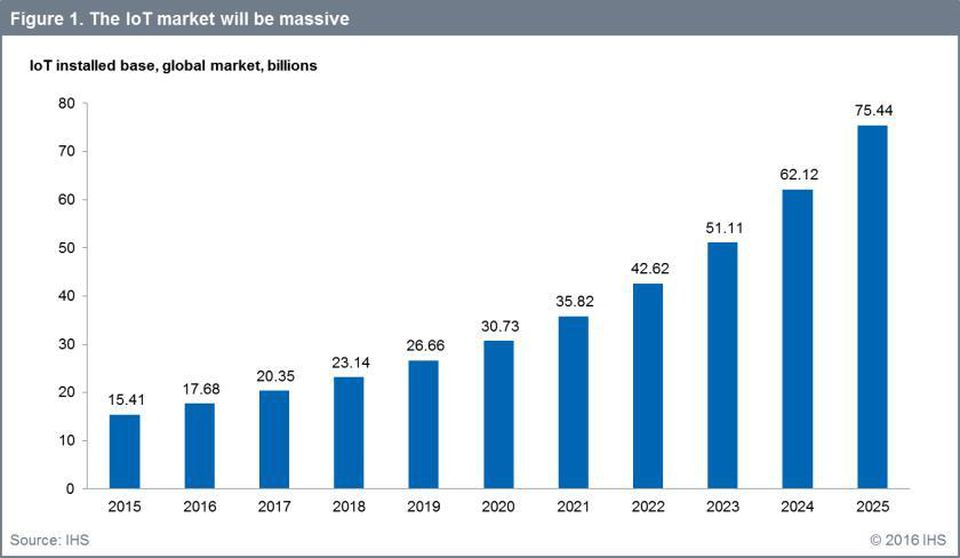
\includegraphics[scale=.4]{iot_growth.jpg}
% figure caption is below the figure
    \caption{IoT Market Growth}
\label{fig:1}       % Give a unique label
\end{figure}
%
% For two-column wide figures use
\begin{figure*}
% Use the relevant command to insert your figure file.
% For example, with the graphicx package use
  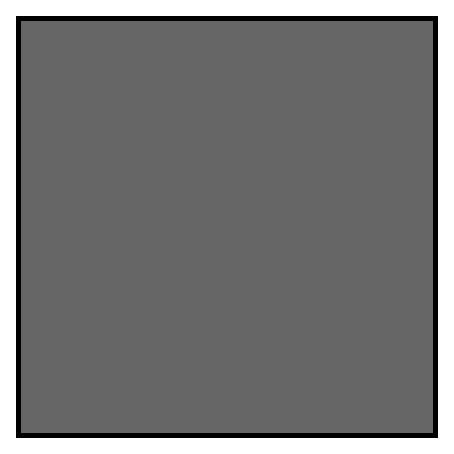
\includegraphics[width=0.75\textwidth]{example.eps}
% figure caption is below the figure
\caption{Please write your figure caption here}
\label{fig:2}       % Give a unique label
\end{figure*}
%
% For tables use
%%\begin{table}
% table caption is above the table
%%\caption{Please write your table caption here}
%%\label{tab:1}       % Give a unique label
% For LaTeX tables use
%%\begin{tabular}{lll}
%%\hline\noalign{\smallskip}
%%first & second & third  \\
%%\noalign{\smallskip}\hline\noalign{\smallskip}
%%number & number & number \\
%%number & number & number \\
%%\noalign{\smallskip}\hline
%%\end{tabular}
%%\end{table}


%\begin{acknowledgements}
%If you'd like to thank anyone, place your comments here
%and remove the percent signs.
%\end{acknowledgements}

% BibTeX users please use one of
%\bibliographystyle{spbasic}      % basic style, author-year citations
%\bibliographystyle{spmpsci}      % mathematics and physical sciences
%\bibliographystyle{spphys}       % APS-like style for physics
%\bibliography{}   % name your BibTeX data base

% Non-BibTeX users please use
\begin{thebibliography}{}
%
% and use \bibitem to create references. Consult the Instructions
% for authors for reference list style.
%
\bibitem{Ref_1}
    Granger, C. W. J. (1969). "Investigating Causal Relations by Econometric Models and Cross-spectral Methods".
\bibitem{Ref_2}
    Diebold, Francis X. (2001). Elements of Forecasting
\bibitem{Ref_3}
     Knight, R. T (2007). "NEUROSCIENCE: Neural Networks Debunk Phrenology". Science
\bibitem{Ref_4}
    Geweke 1982    
\bibitem{Ref_5}
    BIC, (Schwartz 1978)) or the Akaike Information Criterion (AIC, (Akaike 1974)
\bibitem{Ref_6}
    elastic.co/elk-stack, Retrieved 18 October 2018
\bibitem{Ref_7}
    docs.splunk.com/Documentation/Splunk/7.2.0/Search/Aboutpredictiveanalytics, Retrieved 18 October 2018
\bibitem{RefJ}
% Format for Journal Reference
Author, Article title, Journal, Volume, page numbers (year)
% Format for books
\bibitem{RefB}
Author, Book title, page numbers. Publisher, place (year)
% etc
\end{thebibliography}

\end{document}
% end of file template.tex

